
\section{\ref{PS:Q:Feasibility}}

\textit{How can we best re-implement the current Siemens system (\cref{sec:SiemensCase}) as a system where the Wind Power Supervisor and the Park Pilots are decentralized?}\newline\newline

\noindent To answer whether or not the current Siemens system can be fully decentralized, the discussion section of this experiment also contains a discussion with regards to the components analyzed in state of the art, see \cref{cha:stateOfTheArt}. \todo{Why the chapter name ref?}


\subsection{Experiments}

The \ref{PS:Q:Feasibility} problem address the possibility of reimplementing the current Siemens system as a decentralized system. The following experiment aims to investigate if the decentralized solution is able to regulate the power production of each turbine, in order to maintain the global power production setpoint.
%
The experiment has the following procedure:
\begin{enumerate}
	\item Start the system with 10 turbines.
	\item Start the graphical interface described in \cref{sec:graphicalInterface}.
	\item Observe that the global setpoint and the global production line on the graphical interface match.
\end{enumerate}

\subsection{Results}
\label{sec:exp:feasibility}
\begin{figure} [!h]
	\centering
	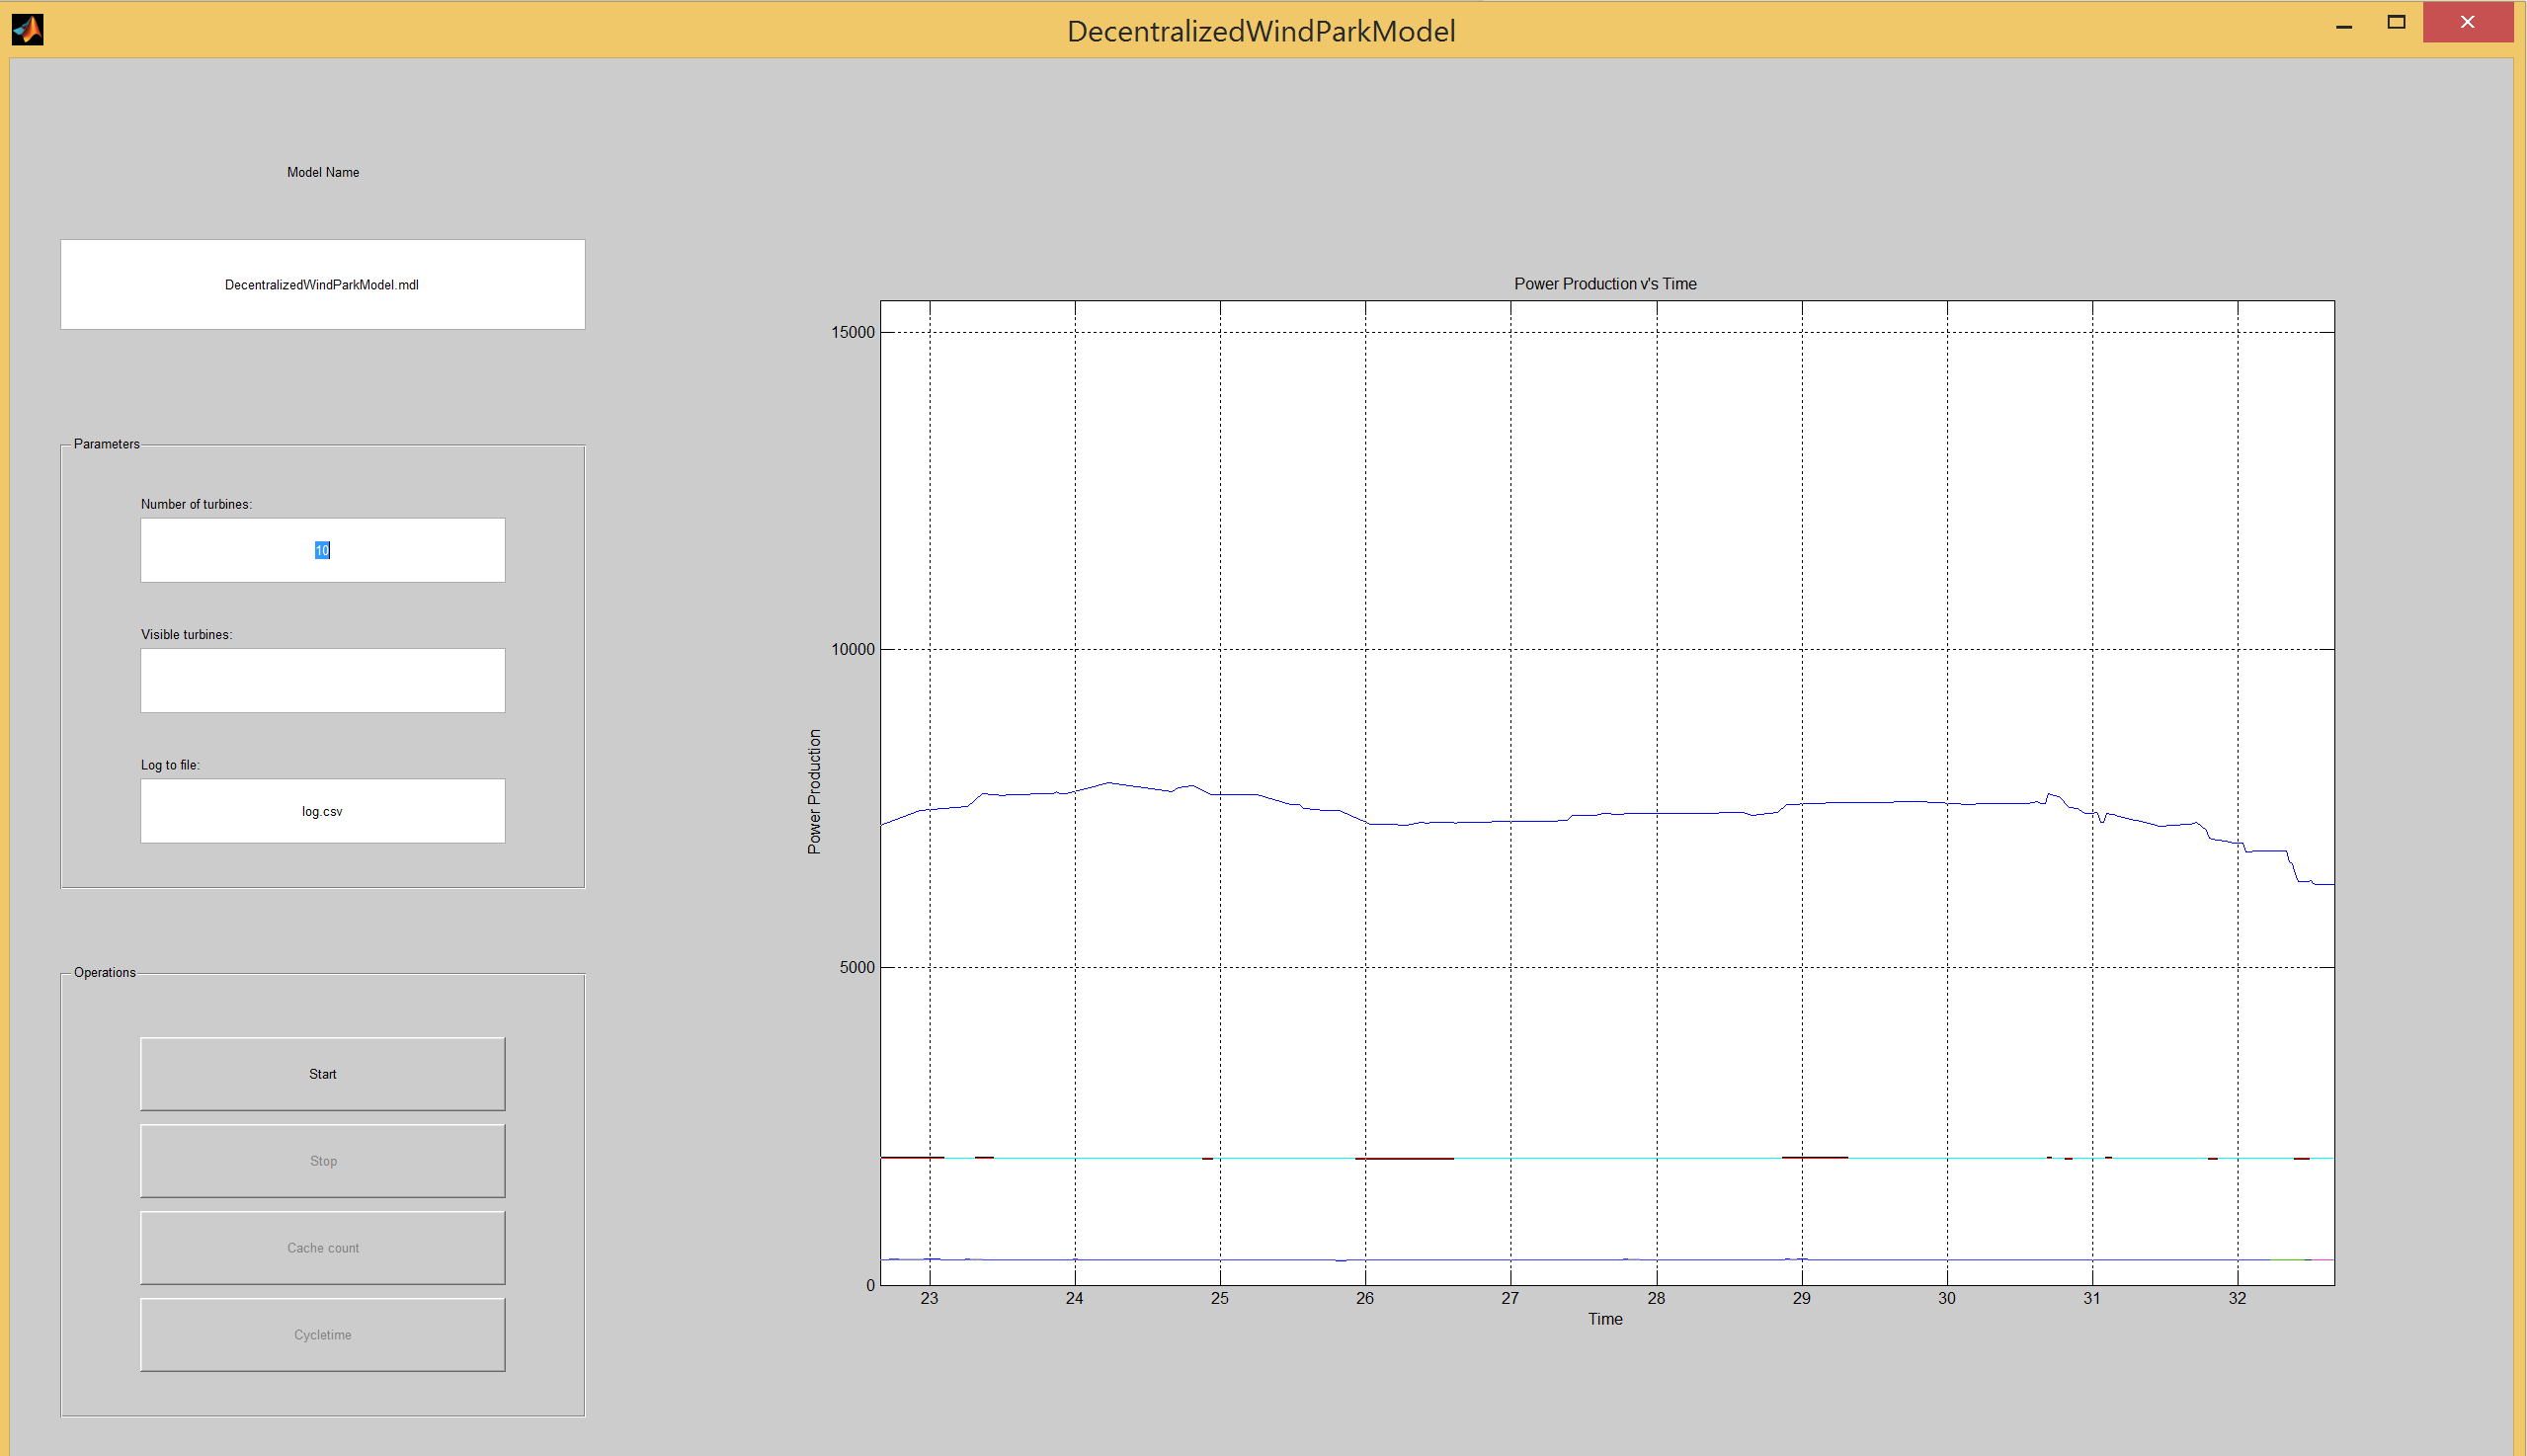
\includegraphics[width=\resultsFigureWidthScale\textwidth]{gui.png} 
	\captionsetup{format=plain,font=footnotesize,labelfont={bf,defaultCapFont},labelsep=quad,singlelinecheck=no}
	\caption[Graphical interface running 10 turbines]{
		\label{fig:graphicalInterface} 
		\footnotesize{%
			Graphical interface running 10 turbines.
		}
	}
\end{figure}

Presented in \cref{fig:graphicalInterface} is a screenshot of the graphical interface made with DDS Blockset for Simulink (described in section \cref{sec:graphicalInterface}). The x-axis show time in seconds and the y-axis show kW production. The screenshot is taken while the decentralized solution runs 10 turbines.
The global setpoint for power production is illustrated by the red line and is showing a value of just below 5000 kW. The global power production is illustrated by the black line also just below 5000 kW.
The blue line illustrates the maximum available power production for the wind farm which, during this experiment, was above 10,000 kW. The lines at the bottom shows values of around 500 kW and they each represents the current power production of each turbine.

\subsection{Discussion}\label{feas:discussion}
The experiment was performed to prove whether or not it is feasible to create a decentralized solution that is able to do power regulation. The experiment consists of a simple run of the prototype of the decentralized solution. The global setpoint and the global production line match and thus we conclude that we have a working prototype, that can regulate according to the global setpoint. Each turbine is expected to produce $globalSetpoint/nTurbines=5000~kW/10=500~kW$(see \cref{sec:calculateSetpoints} for detailed description of the regulation algorithm), which they do. The slight deviation (the deviation that makes each turbine produce close to 500 kW and not exactly 500 kW) is due to the turbine simulating recorded wind conditions and therefore the actual production value change slightly.

As such it is hard to deduce from a screenshot that the decentralized solution is actually able to perform power regulation, but this experiment in correlation with the rest of the experiments performed in this chapter will show that the prototype is working.

To fully decentralize the current Siemens system, decentralization of the Wind Power Supervisor must also be covered. The purpose of the Wind Park Supervisor is to log data from every turbine within the farm and handle external communication. Thus the Wind Park Supervisor consists of tree primary features: Data storage, data aggregation and external communication. 

Decentralizing the data storage and aggregation onto the turbines requires a horizontally scalable distributed database, which can handle data aggregation.
Distributing the database horizontally is important in order to handle datasets larger than the physical storage of one turbine.
Aggregated data is used for generating data suitable for monitoring and analyses.
To handle this MongoDB~\cite{mongodb} has been identified as the optimal component (as concluded in \cref{sec:databaseStorage} Data Storage). MongoDB supports Sharding for horizontal partitioning of datasets and data aggregation across shards. MongoDB has been chosen based on other parameters related to the problem \ref{PS:Q:Availability}, however to answer the \ref{PS:Q:Feasibility} problem, this functionality is sufficient. 

Handling external communication in a decentralized way while still maintaining a single entry point to the system,
requires a solution with multiple nodes capable of sharing this single entry point.
We imagine it done by using multiple Linux Virtual Servers sharing a single virtual IP address (see \cref{cha:resourceManagement}).

\clearpage